\documentclass{article}
\usepackage[utf8]{inputenc}
\usepackage[english]{babel}
\usepackage[]{amsthm} 
\usepackage[]{amssymb} 
\usepackage{amsmath}
\usepackage{graphicx}
\usepackage{stmaryrd}
\usepackage{mdframed}

\title{HW7}
\author{Lo Chun, Chou \\ R13922136}
\date\today

\begin{document}
\setlength{\parindent}{0pt}
\maketitle 

\section*{5.}

uniform blending $2M +1$ binary classifiers $\{g_t\}_{t=1}^{2M+1}$ \\
$\Rightarrow$ aggregation binary classifier:

\begin{equation*}
    G(\mathbf{x}) = \mathrm{sign}\left(\sum_{t=1}^{2M+1} g_t(\mathbf{x})\right)
\end{equation*}

each $g_t$: test $0/1$ error $E_{out}(g_t) = e_t = \mathbb{E}_{\mathbf{x} \sim P}\llbracket g_t(\mathbf{x}) \neq y\rrbracket$
\bigskip

Observe the formulation of $ G(\mathbf{x})$, we can see that:

\begin{equation*}
    G(\mathbf{x}) = 
    \begin{cases}
        1, & \text{if } \#\{g_t(\mathbf{x}) = 1\} \ge M+1 \\
        -1, & \text{if } \#\{g_t(\mathbf{x}) = 1\} \le M \\
    \end{cases}
\end{equation*}

which means that $G(\mathbf{x})$ makes a wrong prediction when $\ge M + 1$ of $g_t(\mathbf{x})$ are wrong.
\bigskip

Let $X_t$ be a $0/1$ indicator variable that outputs $1$ when $g_t(\mathbf{x})$ is wrong, and $0$ otherwise. 
We can write:

\begin{equation*}
    \mathbb{P}(X_t = i) = e_t^i (1 - e_t)^{1-i} \quad ,i \in \{0, 1\}
\end{equation*}

Thus, we have:

$$
\begin{cases}
    \mathbb{P}(X_t = 1) = e_t \\
    \mathbb{P}(X_t = 0) = 1 - e_t
\end{cases}    
$$

If we further let $X$ denote the amount of $g_t(\mathbf{x})$ that are wrong, 
which is equivalent to the amount of $X_t = 1$. 
This makes $X$ a random variable that represents "the amount of $X_t = 1$ in the $2M + 1$ trials".
\bigskip

Since we are asked to not assume the independency among the binary classifier $g_t$s,
the Hoeffding's inequality cannot be used. 
Instead, we can use another inequality that does not restrict independency, the Markov's inequality is as follows:

\begin{mdframed}
Let $Z \ge 0$ be a nonnegative random variable, then for all $t \ge 0$,
\begin{equation*}
    \mathbb{P}(Z \ge t) \le \frac{\mathbb{E}[Z]}{t}
\end{equation*}
\end{mdframed}

In order to calculate this bound, we need to first calculate $\mathbb{E}[X]$, 
which is the expected amount of $X_t = 1$ in the $2M + 1$ trials:

\begin{equation*}
    \mathbb{E}[X] = \sum_{t=1}^{2M+1} \mathbb{E}[X_t] = \sum_{t=1}^{2M+1} e_t
\end{equation*}

substisute back in and we'll get:

\begin{equation*}
\mathbb{P}(X \ge M + 1) \le \frac{1}{M + 1}\sum_{t=1}^{2M+1} e_t
\end{equation*}

\newpage

\section*{6.}

Given:

\begin{equation*}
\begin{split}
    &U_t = \sum_{n=1}^N u_n^{(t)} \quad \text{which means } U_1 = 1 \\
    &\text{assume } 0 < \epsilon_t < \frac{1}{2} \quad \text{for each hypothesis } g_t \\
\end{split}
\end{equation*}

Also, the definition of $\epsilon_t$ is:

\begin{equation*}
    \epsilon_t = \frac{\sum_{n=1}^N u_n^{(t)}\llbracket y_n \neq g_t(x_n) \rrbracket}{\sum_{n=1}^N u_n^{(t)}}
\end{equation*}

Need to show:

\begin{equation*}
    \frac{U_{t+1}}{U_t} = 2\sqrt{\epsilon_t(1-\epsilon_t)}
\end{equation*}

\begin{proof}

The updating rule of $\mathbf{u}^{(t)}$ to $\mathbf{u}^{(t+1)}$ is:

\begin{equation*}
    u_n^{(t+1)} = 
    \begin{cases}
        u_n^{(t)} \sqrt{\frac{1-\epsilon_t}{\epsilon_t}} & \text{if } g_t(x_n) \neq y_n \\
        u_n^{(t)}  \frac{1}{\sqrt{\frac{1-\epsilon_t}{\epsilon_t}}} & \text{if } g_t(x_n) = y_n 
    \end{cases}
\end{equation*}

and we have:

\begin{equation*}
\alpha_t = \ln \left( \sqrt{\frac{1-\epsilon_t}{\epsilon_t}} \right)
\end{equation*}

Therefore, it is equivalent to let:

\begin{equation*}
    u_n^{(t+1)} = 
    \begin{cases}
        u_n^{(t)} e^{\alpha_t} & \text{if } g_t(x_n) \neq y_n \\
        u_n^{(t)} e^{-\alpha_t} & \text{if } g_t(x_n) = y_n 
    \end{cases}
\end{equation*}

Using the fact that $ g_t(x_n)y_n = -1$ for incorrect examples and $ g_t(x_n)y_n = 1$ for correct examples, we can write:

\begin{equation*}
    u_n^{(t+1)} = u_n^{(t)}e^{-\alpha_t g_t(x_n) y_n}
\end{equation*}

Thus, to calculate $U_{t+1}$, we have:

\begin{equation*}
\begin{split}
    U_{t+1} 
    &= \sum_{n=1}^N u_n^{(t+1)} \\
    &= \sum_{n=1}^N u_n^{(t)} e^{-\alpha_t g_t(x_n) y_n} \\
    &= \sum_{n=1}^N u_n^{(t)} \cdot \left[\llbracket y_n \neq g_t(x_n) \rrbracket \exp(\alpha_t) + \llbracket y_n = g_t(x_n) \rrbracket \exp(-\alpha_t)\right]
\end{split}
\end{equation*}

Also, by the definition of $\epsilon_t$, we have:

\begin{equation*}
\begin{split}
\epsilon_t &= \frac{\sum_{n=1}^N u_n^{(t)} \llbracket y_n \neq g_t(x_n) \rrbracket}{\sum_{n=1}^N u_n^{(t)}} = \frac{\sum_{n=1}^N u_n^{(t)} \llbracket y_n \neq g_t(x_n) \rrbracket}{U_t} \\
1 - \epsilon_t &= \frac{\sum_{n=1}^N u_n^{(t)} \llbracket y_n = g_t(x_n) \rrbracket}{U_t}
\end{split}
\end{equation*}

which is equivalent to:

\begin{equation*}
    \sum_{n=1}^N u_n^{(t)} \llbracket y_n \neq g_t(x_n) \rrbracket = \epsilon_t U_t
\end{equation*}

\begin{equation*}
    \sum_{n=1}^N u_n^{(t)} \llbracket y_n = g_t(x_n) \rrbracket = (1 - \epsilon_t) U_t
\end{equation*}

Therefore:

\begin{equation*}
\begin{split}
    U_{t+1} 
    &= \sum_{n=1}^N u_n^{(t)} \llbracket y_n \neq g_t(x_n) \rrbracket \exp(\alpha_t) + \sum_{n=1}^N u_n^{(t)} \llbracket y_n = g_t(x_n) \rrbracket \exp(-\alpha_t) \\
    &= \epsilon_t U_t \exp(\alpha_t) + (1 - \epsilon_t) U_t \exp(-\alpha_t) \\
    &= U_t \cdot \left[\epsilon_t \exp(\alpha_t) + (1 - \epsilon_t) \exp(-\alpha_t)\right] \\
\end{split}
\end{equation*}

and

\begin{equation*}
\begin{split}
    \frac{U_{t+1}}{U_t} 
    &= \epsilon_t \exp(\alpha_t) + (1 - \epsilon_t) \exp(-\alpha_t) \\
    &= \epsilon_t \sqrt{\frac{1-\epsilon_t}{\epsilon_t}} + (1 - \epsilon_t) \sqrt{\frac{\epsilon_t}{1-\epsilon_t}} \\
    &= \sqrt{\epsilon_t(1-\epsilon_t)} + \sqrt{\epsilon_t(1-\epsilon_t)} \\
    &= 2\sqrt{\epsilon_t(1-\epsilon_t)}
\end{split}
\end{equation*}

\end{proof}

\newpage

\section*{7.}

In the original gradient boosting, the update rule is:

\begin{equation*}
    \theta^{(k)} = \theta^{(k-1)} + \alpha_k T_k
\end{equation*}

In this problem, we are asked to use linear regression (without regularization) to replace decision trees, which means:

\begin{equation*}
    \theta^{(k)} = \theta^{(k-1)} + \alpha_k \mathrm{LR}_k
\end{equation*}

where $\mathrm{LR}_k$ is defined as follows:

\begin{equation*}
    \mathrm{LR}_k(X) = X \mathbf{w}_k
\end{equation*}

where $X \in \mathbb{R}^{N \times d}$ is the feature matrix, 
and $\mathbf{w}_k \in \mathbb{R}^d$ is the weight vector at iteration $k$.

To find $\mathbf{w}_k$, we fit the residuals $\mathbf{r}^{(k)}$, which is calculated by:

\begin{equation*}
    \mathbf{r}^{(k)} = \mathbf{y} - \hat{\mathbf{y}}^{(k-1)}
\end{equation*}

where $\hat{\mathbf{y}}^{(k-1)} = X \hat{\mathbf{w}}^{(k-1)}$ is the prediction of the previous iteration.

Thus, we find $\mathbf{w}_k$ by using least squares:

\begin{equation*}
    \mathbf{w}_k = (X^T X)^{-1} X^T \mathbf{r}^{(k)}
\end{equation*}

and we can rewrite $\mathrm{LR}_k(X)$ as:

\begin{equation*}
    \mathrm{LR}_k(X) = X (X^T X)^{-1} X^T \mathbf{r}^{(k)}
\end{equation*}

To check if $\alpha_1 = 1$ is optimal, we need to check if it results in a minimized error 
(using the model $\theta^{(1)}$)
\bigskip

If we assume the prediction of the initial model is $\theta^{(0)}(X) = X\mathbf{w}_0$, 
then prediction of $\theta^{(1)}$ is:

\begin{equation*}
\begin{split}
    \theta^{(1)}(X) 
    &= \theta^{(0)}(X) + \alpha_1 \mathrm{LR}_1(X) \\
    &= X\mathbf{w}_0 + \alpha_1 X (X^T X)^{-1} X^T \mathbf{r}^{(1)} \\
\end{split}
\end{equation*}

and the loss incured in iteration $1$ is:

\begin{equation*}
\begin{split}
    \left\| \mathbf{y} - \theta^{(1)}(X) \right\|^2 
    &= \left\| \mathbf{y} - X\mathbf{w}_0 - \alpha_1 X(X^T X)^{-1} X^T \mathbf{r}^{(1)} \right\|^2 \\
    &= \left\| \mathbf{r}^{(1)} - \alpha_1 X(X^T X)^{-1} X^T \mathbf{r}^{(1)} \right\|^2 \\
    &= \left(\mathbf{r}^{(1)} - \alpha_1 X(X^T X)^{-1} X^T \mathbf{r}^{(1)}\right)^T \left(\mathbf{r}^{(1)} - \alpha_1 X(X^T X)^{-1} X^T \mathbf{r}^{(1)}\right) \\
    &= \mathbf{r}^{(1)T} \mathbf{r}^{(1)} - 2\alpha_1 \mathbf{r}^{(1)T} X(X^T X)^{-1} X^T \mathbf{r}^{(1)} + \alpha_1^2 \mathbf{r}^{(1)T} X(X^T X)^{-1} X^T X(X^T X)^{-1} X^T \mathbf{r}^{(1)} \\
    &= \mathbf{r}^{(1)T} \mathbf{r}^{(1)} - 2\alpha_1 \mathbf{r}^{(1)T} X(X^T X)^{-1} X^T \mathbf{r}^{(1)} + \alpha_1^2 \mathbf{r}^{(1)T} X(X^T X)^{-1} X^T \mathbf{r}^{(1)} \\
\end{split}
\end{equation*}

Taking the derivative w.r.t. $\alpha_1$ and set it to $0$, we have:

\begin{equation*}
\begin{split}
    &\frac{d}{d\alpha_1} \left(\mathbf{r}^{(1)T} \mathbf{r}^{(1)} - 2\alpha_1 \mathbf{r}^{(1)T} X(X^T X)^{-1} X^T \mathbf{r}^{(1)} + \alpha_1^2 \mathbf{r}^{(1)T} X(X^T X)^{-1} X^T \mathbf{r}^{(1)}\right) = 0 \\
    &\Rightarrow -2 \mathbf{r}^{(1)T} X(X^T X)^{-1} X^T \mathbf{r}^{(1)} + 2\alpha_1 \mathbf{r}^{(1)T} X(X^T X)^{-1} X^T \mathbf{r}^{(1)} = 0 \\
    &\Rightarrow \alpha_1 = \frac{2 \mathbf{r}^{(1)T} X(X^T X)^{-1} X^T \mathbf{r}^{(1)}}{2\mathbf{r}^{(1)T} X(X^T X)^{-1} X^T \mathbf{r}^{(1)}}\\
    &\Rightarrow \alpha_1 = 1
\end{split}
\end{equation*}

Therefore, $\alpha_1 = 1$ is optimal.

\newpage

\section*{8.}

After updating all $s_n$ in iteration $t$, using the steepest $\eta$ as $\alpha_t$ need to prove that:

\begin{equation*}
    \sum_{n=1}^N (y_n -s_n^{(t)})g_t(\mathbf{x}_n) = 0
\end{equation*}

\begin{proof}
At iteration $t$, since $\alpha_t = \eta_t$, we update the model by:

\begin{equation*}
    \theta^{(t+1)} = \theta^{(t)} + \eta_t g_t
\end{equation*}

To update individual predictions $s_n^{(t)}$, we have:

\begin{equation*}
    s_n^{(t)} = s_n^{(t-1)} + \eta_t g_t(\mathbf{x}_n)
\end{equation*}

To obtain $g_t$, we need to train it by fitting the residuals:

\begin{equation*}
    r_n^{(t)} = y_n - s_n^{(t-1)}
\end{equation*}

so that $g_t$ minimizes the loss:

\begin{equation*}
    \sum_{n=1}^N \left(r_n^{(t)} - g_t(\mathbf{x}_n)\right)^2 = \sum_{n=1}^N \left(y_n - s_n^{(t-1)} - g_t(\mathbf{x}_n)\right)^2 
\end{equation*}

Thus, we take the derivative w.r.t. $g_t$ and set it to $0$, and we'll have:

\begin{equation*}
\begin{split}
    &\frac{d}{dg_t} \sum_{n=1}^N \left(y_n - s_n^{(t-1)} - g_t(\mathbf{x}_n)\right)^2 = 0 \\
    &\Rightarrow -2 \sum_{n=1}^N \left(y_n - s_n^{(t-1)} - g_t(\mathbf{x}_n)\right) = 0 \\
    &\Rightarrow \sum_{n=1}^N \left(y_n - s_n^{(t-1)} - g_t(\mathbf{x}_n)\right) = 0 \\
    &\Rightarrow \sum_{n=1}^N \left(y_n - s_n^{(t-1)}\right) = \sum_{n=1}^N g_t(\mathbf{x}_n) \\
    &\Rightarrow \sum_{n=1}^N r_n^{(t)} = \sum_{n=1}^N g_t(\mathbf{x}_n) \\
\end{split}
\end{equation*}

The original equation that we want to prove can then be derived as follows:

\begin{align*}
    \sum_{n=1}^N (y_n -s_n^{(t)})g_t(\mathbf{x}_n) 
    &= \sum_{n=1}^N \left(y_n - s_n^{(t-1)} - \eta_t g_t(\mathbf{x}_n)\right)g_t(\mathbf{x}_n) \\
    &= \sum_{n=1}^N \left(r_n^{(t)} - \eta_t g_t(\mathbf{x}_n)\right)g_t(\mathbf{x}_n) \\
    &= \sum_{n=1}^N r_n^{(t)} g_t(\mathbf{x}_n) - \eta_t \sum_{n=1}^N g_t(\mathbf{x}_n)^2 \tag{*} 
\end{align*}

By lecture note 11, p.19, we have:

\begin{equation*}
    \frac{\sum_{n=1}^N g_t(\mathbf{x}_n)(y_n - s_n^{(t-1)})}{\sum_{n=1}^N g_t(\mathbf{x}_n)^2} 
    = \arg \min_{\eta} \frac{1}{N} \sum_{n=1}^N \left((y_n - s_n^{(t-1)}) - \eta g_t(\mathbf{x}_n)\right)^2
\end{equation*}

Thus, by plugging in this result into equation $(*)$, we have:

\begin{align*}
    &\sum_{n=1}^N (y_n -s_n^{(t)})g_t(\mathbf{x}_n) \\
    &= \sum_{n=1}^N r_n^{(t)} g_t(\mathbf{x}_n) - \frac{\sum_{n=1}^N g_t(\mathbf{x}_n)(y_n - s_n)}{\sum_{n=1}^N g_t(\mathbf{x}_n)^2} \sum_{n=1}^N g_t(\mathbf{x}_n)^2 \\ 
    &= \sum_{n=1}^N r_n^{(t)} g_t(\mathbf{x}_n) - \sum_{n=1}^N g_t(\mathbf{x}_n)(y_n - s_n^{(t-1)}) \\
    &= \sum_{n=1}^N r_n^{(t)} g_t(\mathbf{x}_n) - \sum_{n=1}^N r_n^{(t)} g_t(\mathbf{x}_n) \\
    &= 0
\end{align*}

\end{proof}

\newpage

\section*{9.}

Initially, for the neurons $j$ and $j+1$ in the hidden layer, we have:

\begin{equation*}
    z_j = \sum_{i=1}^d w_{ij}^{(1)} x_i + b_j^{(1)}, \quad z_{j+1} = \sum_{i=1}^d w_{i,j+1}^{(1)} x_i + b_{j+1}^{(1)}
\end{equation*}

and the outputs are:

\begin{equation*}
h_j = \tanh(z_j), \quad h_{j+1} = \tanh(z_{j+1})
\end{equation*}

Since all the initial weights $w_{i,j}^{l} = 0.5$

\newpage

\section*{10.}

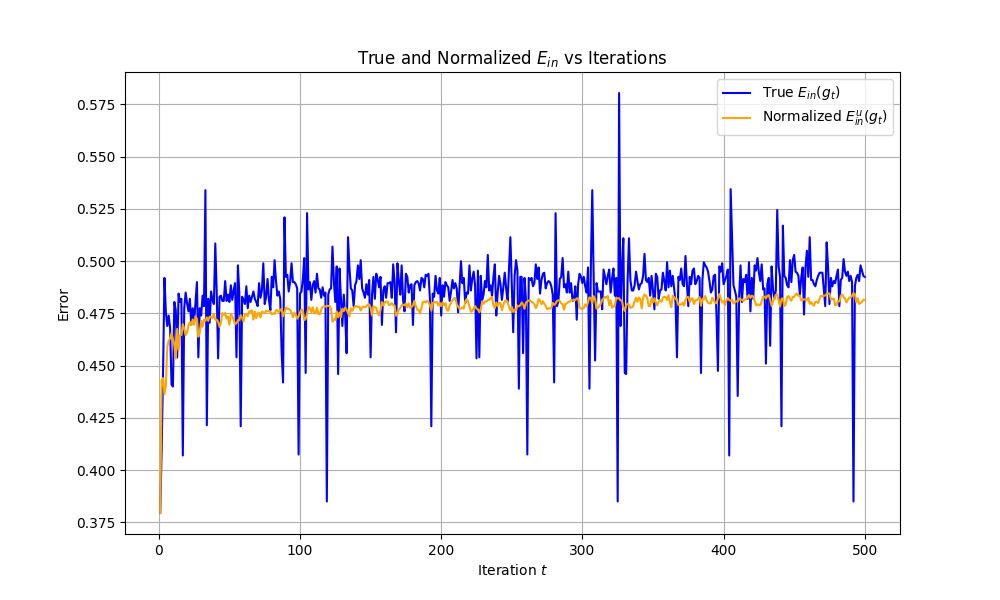
\includegraphics[width = \textwidth, height = \textheight, keepaspectratio]{10_v6_result.png}

From this plot we can see that, the true $E_{in}$ (the blue curve) fluctuates greatly, 
this may due to the fact that AdaBoost place emphasis on the misclassified examples by adding more weights on them,
since focusing on specific examples can bring instability in the performance of individual weak learners. \\

The normalized $E_{in}^u$ (the orange curve) measures the weighted error.
While AdaBoost adjusts weights to focus more on the misclassified examples at each iteration,
this weighted error reflects how well the weak learner is performing on those examples.\\

\newpage


\includegraphics[width = 0.5\textwidth, keepaspectratio]{10_v6_snapshot_1.png}

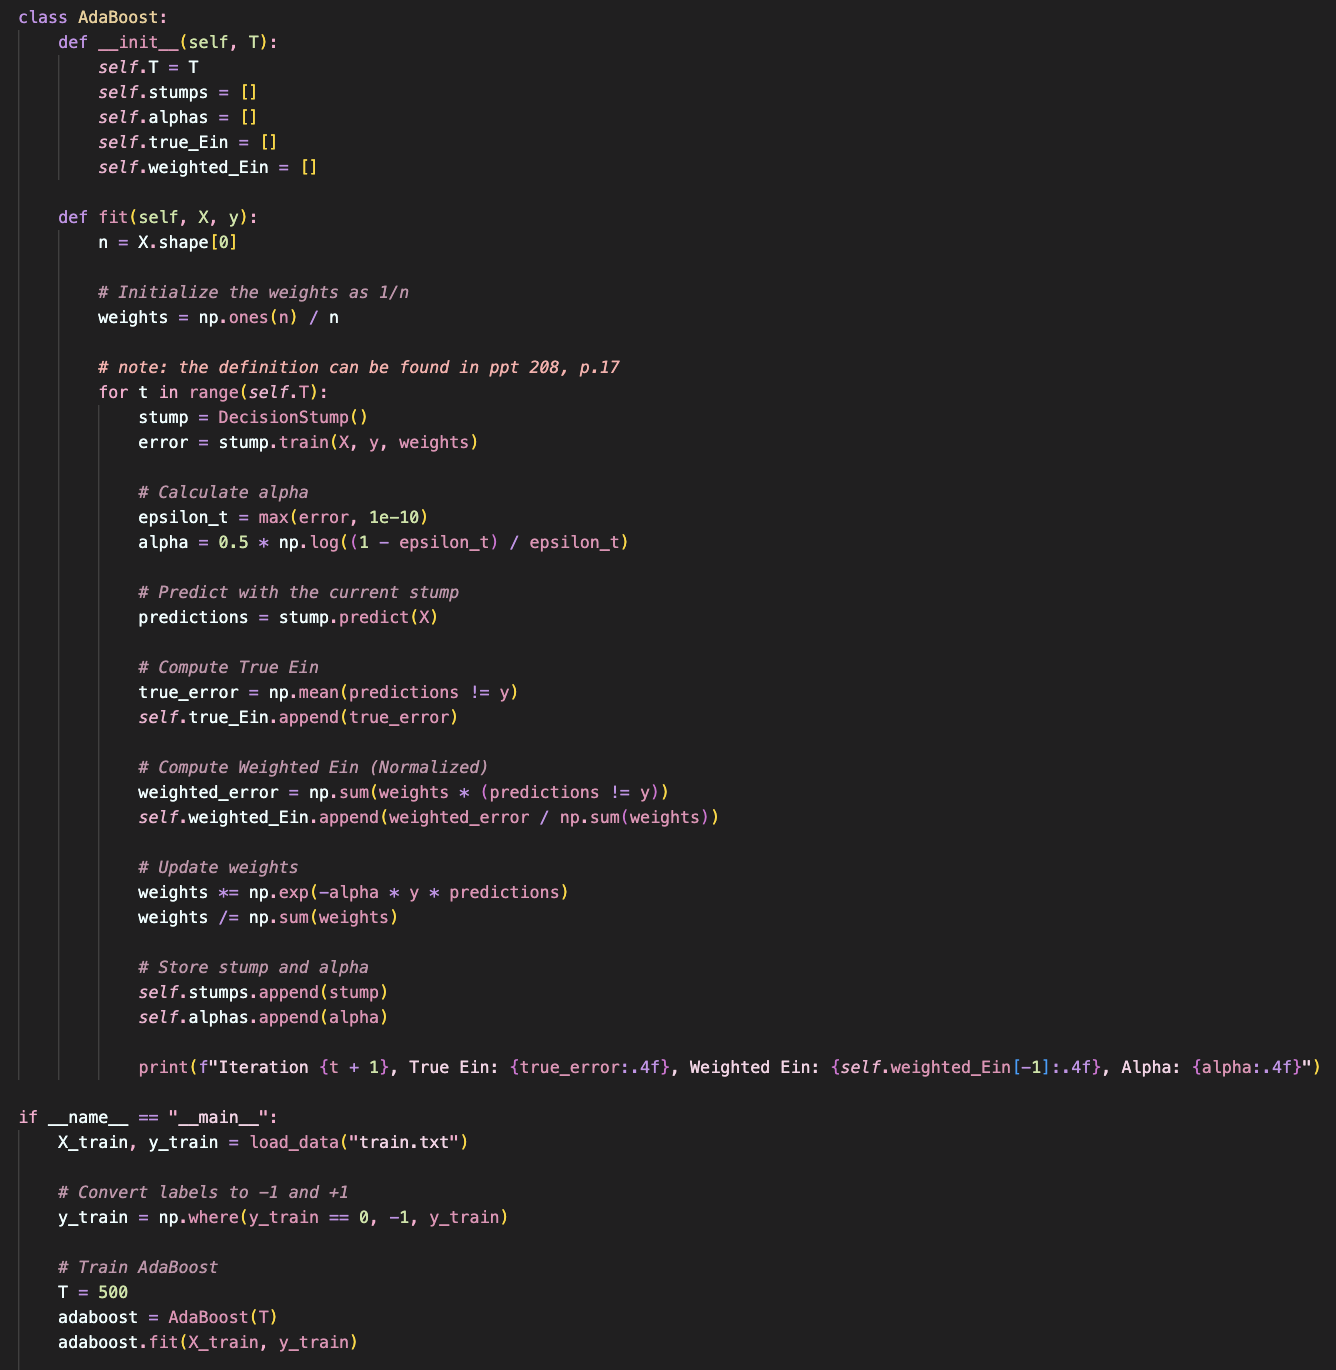
\includegraphics[width = 0.5\textwidth, keepaspectratio]{10_v6_snapshot_2.png}


\newpage

\section*{11.}

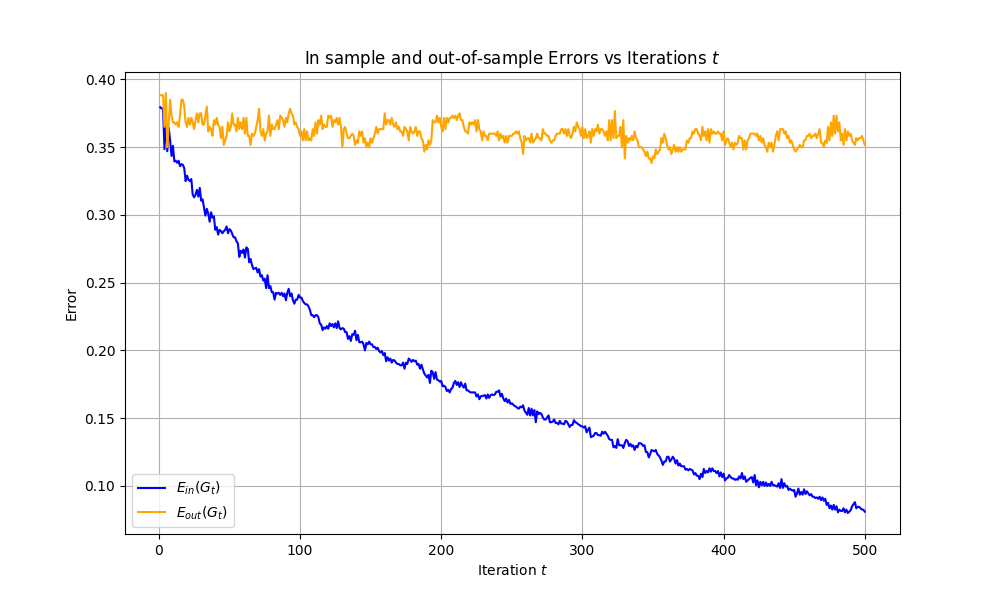
\includegraphics[width = \textwidth, height = \textheight, keepaspectratio]{11_result_1112.png}

From the above figure, we can see that 
the blue curve (which is the in sample error), shows that $E_{in}$ decreases steadily as the number of iterations $t$ increases.
When we got to $T = 500$, the error is quite low, which matches our expectation since
the target of AdaBoost is to iteratively minimize the training error by giving the misclassified exampels higher weights.
Therefore, the model becomes increasingly fitted to the training data.
\newline

For the orange curve (which is the out-of-sample error), shows that even though the curve fluctuates,
after we got to $T = 500$, it did not decrease like $E_in$ does. 
This implies that our model is not generalizing well, and this result is as expected,
since as we make the model more fitted to the training data, overfitting must happen.

\newpage

\section*{12.}

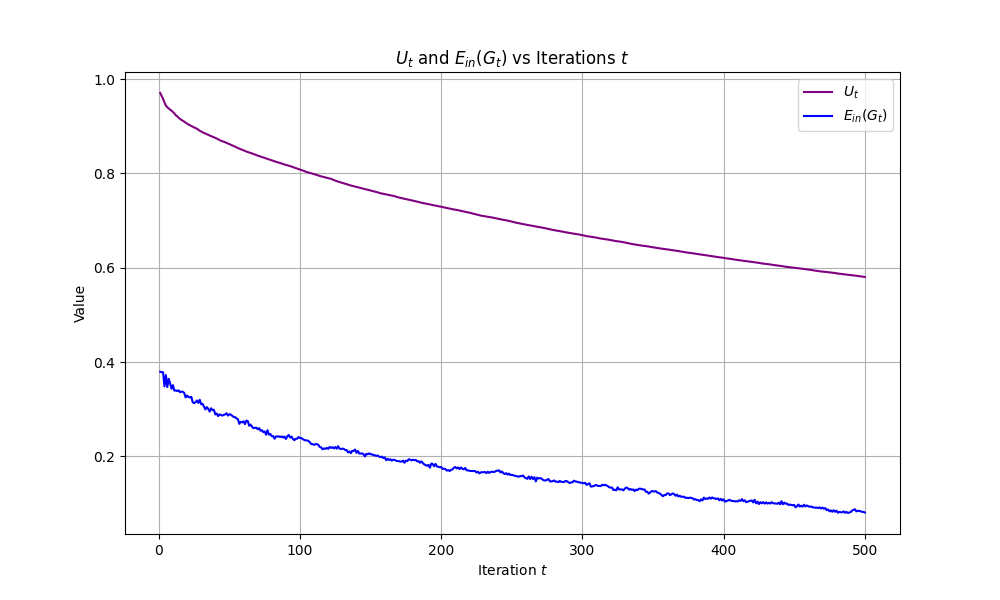
\includegraphics[width = \textwidth, height = \textheight, keepaspectratio]{12_result_1112.png}

The purple curve (which represents the sum of weights $U_t$) is steadily decreasing as the iteration number decreases.
We can see that initially, this value matches the definition that all weights are $\frac{1}{n}$, and therefore making the sum to be $1$. \\

The decreased result also matches our expectation, since if the weak learners consistently achieve errors $ \epsilon_{\tau} < 0.5$, 
the value $U_t$ keeps decreasing. 
Moreover, as the value of $\epsilon_{\tau}$ becomes smaller, the decreasing behavior should slow down,
and this can also be seen in our plot.
\newline

From the blue curve, we can see that $E_{in}(G_t)$ is also steadily decreasing.
This shows that $U_t$ and $E_{in}(G_t)$ have similar behavior as the number of iteration increases.
The reason why $E_{in}(G_t)$ is decreasing is that when we add more weak classifiers to our model, 
it becomes stronger, hence having the ability to fit the examples better, and thus reduces the error value.  

\newpage

\section*{13.}

From the reply of ChatGPT, it said that:
\bigskip

For $3$ input bits $(x_1, x_2, x_3)$, the hidden neuron could compute:

\begin{align*}
h_1 &= x_1 \oplus x_2 \\
h_2 &= h_1 \oplus x_3 \\
\end{align*}

To see how many neurons is required to implement the $XOR$ function for $d = 3$, 
we first consider the implementation of the $XOR$ function for $d = 2$, which is:

\begin{align*}
h_1 &= x_1 \oplus x_2 \\
\end{align*}

From the property that $XOR$ can be implemented using $AND$ and $OR$ gates, which is:

\begin{equation*}
A \oplus B = ( \bar{A} \cdot B) + (A \cdot \bar{B})
\end{equation*}

we can obtain $h_1$ by using $2$ neurons, which are the two terms in the following equation:

\begin{equation*}
h_1 = ( \bar{x}_1 \cdot x_2) + (x_1 \cdot \bar{x}_2) \\
\end{equation*}

Using this result and getting back to the $XOR$ function for $d = 3$, we have:

\begin{align*}
    x_1 \oplus x_2 \oplus x_3
    &= (x_1 \oplus x_2) \oplus x_3 \\
    &= (\bar{x}_1 \cdot x_2 + x_1 \cdot \bar{x}_2) \oplus x_3 \\
    &= \overline{(\bar{x}_1 \cdot x_2 + x_1 \cdot \bar{x}_2)} \cdot x_3 + (\bar{x}_1 \cdot x_2 + x_1 \cdot \bar{x}_2) \cdot \bar{x}_3 \\
    &= (\overline{\bar{x}_1 \cdot x_2} \cdot \overline{x_1 \cdot \bar{x}_2}) \cdot x_3 + (\bar{x}_1 \cdot x_2 + x_1 \cdot \bar{x}_2) \cdot \bar{x}_3 \\
    &= (x_1 + \bar{x}_2) \cdot (\bar{x}_1 + x_2) \cdot x_3 + (\bar{x}_1 \cdot x_2 + x_1 \cdot \bar{x}_2) \cdot \bar{x}_3 \\
    &= x_1\bar{x}_1x_3 + x_1x_2x_3 + \bar{x}_1\bar{x}_2x_3 + \bar{x}_2x_2x_3 + \bar{x}_1x_2\bar{x}_3 + x_1\bar{x}_2\bar{x}_3 \\
    &= x_1x_2x_3 + \bar{x}_1\bar{x}_2x_3 + \bar{x}_1x_2\bar{x}_3 + x_1\bar{x}_2\bar{x}_3 \\
\end{align*}

By this result, we can see that four neurons are required for the case $d = 3$.
Hence, we have $2-2-1$ for two input bits, and $3-4-1$ for three input bits,
if we observe the result, we can find that we need:

\begin{itemize}
    \item one term for all of the input bits are not inverted (i.e. $x_1x_2x_3$ in this example)
    \item $d$ terms for each input bit not inverted, and others inverted (i.e. $x_1\bar{x}_2\bar{x}_3, \ \bar{x}_1x_2\bar{x}_3, \ \bar{x}_1\bar{x}_2x_3$)
\end{itemize} 

Therefore, to implement a $XOR$ function on $d$ input bits,
we need $d + 1$ neurons in the hidden layer, which shows the insufficiency for using $d-1$ neurons.

\end{document}